
\documentclass{article}
\usepackage{tikz}
\title{Problem Set 1}
\date{CSC263 2026 Winter}

\begin{document}
This problem set covers heaps, BSTs, and AVL trees.  You can use data structures from class as builtins. On some questions it may be helpful to modify one of these data structures (by storing an additional value, for example). You do not have to give full pseudocode for the modified data structure but you should give enough pseudocode that you can support your runtime claims. 

The points don't correspond to the difficulty. A star after the point value indicates that I think the question is harder than the others.
\begin{enumerate}

	\item \textbf{[8]} Give pseudocode for a function tree-range(bst, min, max) that returns the sum of all values in bst between min and max, inclusive. 

		Your algorithm should run in $O(n)$ time. We may deduct points for inefficiency even if it doesn't impact the asymptotic runtime - you should visit as few nodes in bst as possible.

		\begin{enumerate}
			\item \textbf{[4]} Pseudocode
			\item \textbf{[4]} Prove that your algorithm visits all nodes with values between min and max.
		\end{enumerate}

	\item \textbf{[8]} Design a data structure that supports two operations, insert and find-median. Insert(x) should run in $O(\log n)$ time, where $n$ is the number of items that have been inserted. Find-median should return the $\lceil(n/4)\rceil^{th}$ largest item that has been inserted, and should run in $O(1)$ time.

	\begin{enumerate}
		\item \textbf{[4]} Pseudocode
		\item \textbf{[4]} Runtime analysis
	\end{enumerate}

\item \textbf{[16]} Design and implement a data structure that supports two opertations, insert and kmin. 
	Insert and kmins should run in $O(\log n)$ time, where $n$ is the number of items that have been inserted.  kmins should return the $i^{th}$ smallest item that has been inserted, where $i$ is the number of times kmins has been called. 

			You will be tested only on the solve\_kmins function. solve\_kmins takes a list of commands as input. A command is a string, either `insert ' followed by a number, or 'kmin'. You will not be tested on any other inputs. Output should be a list containing the return values of each call to kmin.

			For example, solve\_kmins([``insert 9'', ``insert 3'', ``kmin'', ``kmin'', ``insert 1'', ``insert 12'', ``kmin'', ``kmin'']) should return [3, 9, 9, 12]. 

			\begin{enumerate}
				\item \textbf{[4]} Give pseudocode for your data structure.
				\item \textbf{[12]}
		Code it up and submit in kmins.py. Some starter code is provided; you will have to implement any data structures yourself.
			\end{enumerate}



	\item {\bf [6]} What's the minimum number of rotations needed to make this an AVL tree (i.e. have balance factor between 1 and -1 for all nodes)?

			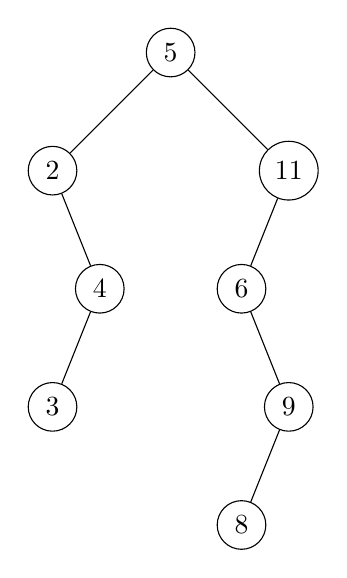
\begin{tikzpicture}
				[level 1/.style={sibling distance=30mm},
				level 2/.style={sibling distance=12mm}]
				\node[circle,draw] {5}
					child{ node[circle,draw] {2}
						child[missing]
						child{ node[circle,draw] {4}
							child{ node[circle,draw] {3}}
							child[missing]
						}
					}
					child{ node[circle,draw] {11}
						child{ node[circle,draw] {6}
						child[missing]
						child{ node[circle,draw] {9}
							child{ node[circle,draw] {8}
							}
							child[missing]
							}
						}
						child[missing]
					};
			\end{tikzpicture}

		Prove it by:
\begin{enumerate}
	\item {\bf[2]} Give a sequence of rotations that AVL-ifies the tree (you can just list them like ``5 R, 3 L, ...'' for right rotation at the node containing 5 then left rotation at the node containing 3). 
	\item {\bf[4*]} Prove it's not possible to balance with fewer rotations.
\end{enumerate}
\end{enumerate}
\end{document}
